% Inspired by - https://tex.stackexchange.com/a/335355

\documentclass[tikz, border=10pt]{standalone}
\usepackage{tikz}
\begin{document}

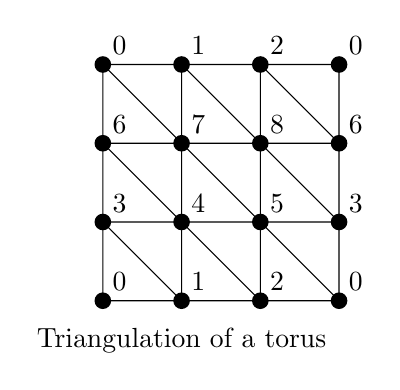
\begin{tikzpicture}
    \node at (1, -0.5) {Triangulation of a torus};
    \draw
        (0, 0) grid[step=1cm] (3, 3)
        (1, 0) -- (0, 1)
        (2, 0) -- (0, 2)
        (3, 0) -- (0, 3)
        (3, 1) -- (1, 3)
        (3, 2) -- (2, 3);
    \fill[radius=3pt]
        \foreach \x in {0, ..., 3} {
            \foreach \y in {0, ..., 3} {
                (\x, \y) circle[]
            }
        };
    \path[above right]
        \foreach \p/\v in {
            {0, 0}/0,
            {1, 0}/1,
            {2, 0}/2,
            {3, 0}/0,
            {0, 1}/3,
            {1, 1}/4,
            {2, 1}/5,
            {3, 1}/3,
            {0, 2}/6,
            {1, 2}/7,
            {2, 2}/8,
            {3, 2}/6,
            {0, 3}/0,
            {1, 3}/1,
            {2, 3}/2,
            {3, 3}/0
        } {
            (\p) node {$\v$}
        };
\end{tikzpicture}
\end{document}
